\documentclass[a4paper,12pt]{jarticle}
\usepackage{listings}
\title{平成26年度 3回生後期学生実験エージェント \\ 課題1}
\author{竹田創)}
\date{提出日:\today  \\ }
%%
\makeatletter

\makeatother
%%
\begin{document}
\maketitle

\section{プログラム概要}
\lstset{numbers=left,basicstyle=\small}
SVM.ccは2次計画問題をとくライブラリ(QuadProg++)と、データとクラスの学習データを元にしてサポートベクタマシンを作成するプログラムである。
\section{外部仕様}

\subsection{プログラム名とファイルの説明}

QuadProg++.ccやQuadProg++.hhは2次計画問題をとくためのライブラリのプログラムである。
sample\_linear.datとsample\_circle.datはデータとクラスの学習データのプログラムである。
1\_circle.dat,a\_linear.dat,minus\_1\_circle.dat,minus\_1\_linear.datは
SVM.ccはサポートベクターマシンを実現するプログラムである。

\lstinputlisting{SVM.cc}

%%
\subsection{プログラム引数の説明}
コンパイルしたファイルを実行するときにコマンドライン引数としてG、Pまたはなにもなしをとる。
Gをとったときはガウスカーネルで計算して、Pをとったときは多項式カーネルで計算し、なにもとらなかったときはカーネルトリックなしで計算する。

%%
\subsection{入出力ファイル及び参照ファイル}
sample\_linear.datとsample\_circle.datはデータとクラスの学習データのプログラムである。
このデータをよみとってSVMを作成する。
また出力結果としてalphaの組を出力する。
%%
\section{コンパイル方法}
\begin{verbatim}
g++-4.7 -Wall QuadProg++.cc SVM.cc
./a.out 
./a.out G
./a.out P

\end{verbatim}

\subsection{実行例}
\begin{verbatim}
alpha
0	0.000000
1	-0.000000
2	0.000000
3	0.000000
4	-0.000000
5	0.000000
6	0.000000
7	-0.000000
8	0.000000
9	-0.000000
10	0.000000
11	-0.000000
12	0.000000
13	0.000000
14	0.000000
15	0.000000
16	0.000000
17	0.000000
18	0.000000
19	0.000000
20	14.900113
21	0.000000
22	6.462795
23	-0.000000
24	0.000000
25	126.382013
26	86.638915
27	0.000000
28	-0.000000
29	-0.000000
30	41.650582
31	0.000000
32	0.000000
33	0.000000
34	-0.000000
35	-0.000000
36	0.000000
37	0.000000
38	-0.000000
39	-0.000000
40	0.000000
41	0.000000
42	0.000000
43	-0.000000
44	0.000000
45	-0.000000
46	-0.000000
47	0.000000
48	129.805469
49	-0.000000
50	8.902141
51	0.000000
52	-0.000000
53	-0.000000
54	-0.000000
55	6.116575
56	-0.000000
57	-0.000000
58	0.000000
59	0.000000
60	-0.000000
61	-0.000000
62	-0.000000
63	0.000000
64	0.000000
65	0.000000
66	-0.000000
67	0.000000
68	-0.000000
69	-0.000000
70	0.000000
71	0.000000
72	7.242414
73	-0.000000
74	0.000000
75	0.000000
76	-0.000000
77	-0.000000
78	0.000000
79	0.000000
80	0.000000
81	80.888327
82	0.000000
83	0.000000
84	-0.000000
85	-0.000000
86	0.000000
87	0.000000
88	0.000000
89	0.000000
90	-0.000000
91	-0.000000
92	-0.000000
93	-0.000000
94	-0.000000
95	0.000000
96	43.959578
97	0.000000
98	2.340770
99	0.000000
weight[0]=12.9251
weight[1]=-177.845
theta=-2285.13
\end{verbatim}
%%
\section{内部仕様}
サポートベクタマシンを実現するSVM.ccについて説明する。
QuadProg++を利用して2次計画問題をとくため、G、CE、CI、g0、ce0、ci0に適切な値を代入する。
CIは単位行列、CEは(y1 y2 y3 ..)という行列、ci0とce0は全ての成分が0のベクトル、g0は全ての成分が-1のベクトルである。行列GはG[i][j]がy[i]*y[j]*Kernel(xi,xj)の成分をもつ行列である。

\section{評価結果}
線形のデータはカーネルトリックなしのときと多項式カーネルのときでうまくとけていることが分かった。
ガウスカーネルのgnuplotで出力がうまくいかなかった。
\begin{figure}[tp]
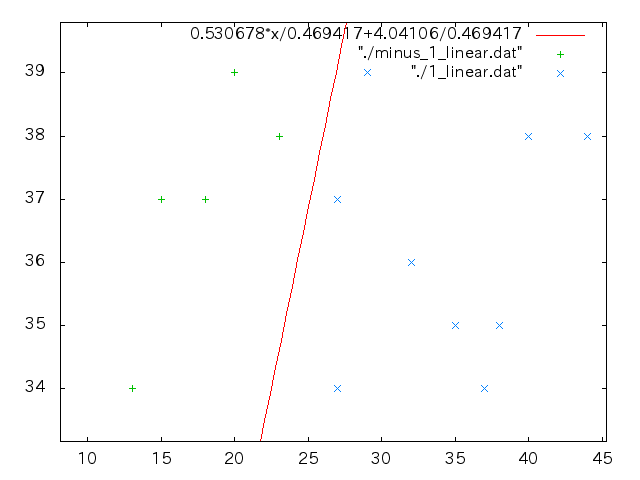
\includegraphics[scale=0.8]{linearNokernel.png}

\caption{線形のデータをカーネルトリックなしで解析}
\label{fig:sample}
\end{figure}



\begin{figure}[tp]
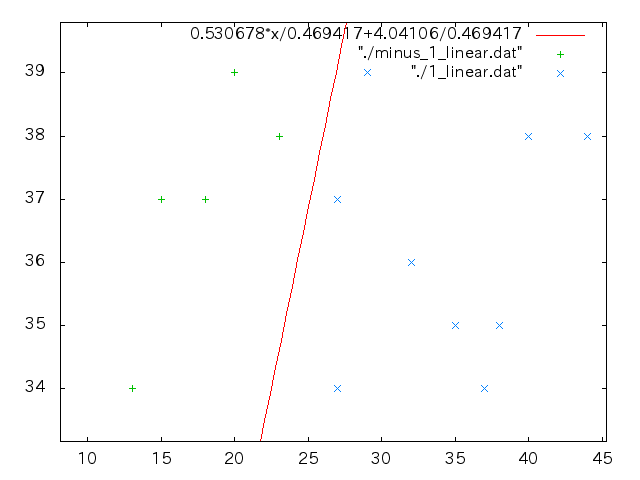
\includegraphics[scale=0.8]{linearPolinomical.png}

\caption{線形のデータを多項式カーネルで解析}
\label{fig:sample}
\end{figure}


\section{考察}
まだガウスカーネルの場合の描画ができていません。
後日実装できしだい再提出します。

%%

\end{document}
























































































































